% !TeX root = orbits.tex

\section{Ellipses in Euclidean geometry}\label{s.geometry}

The proofs of theorems about planetary freely used analytic geometry and trigonometry, but for many years after the invention of analytic geometry, mathematicians continued to limit themselves to Euclidean geometry. Even into the late nineteenth century, students continued to study the original works of Euclid and Newton. In this section, I present proofs in Euclidean geometry (\emph{geometric proofs}) of theorems that appeared in the previous sections. The proofs are based on the definition of ellipses in terms of the geometric concepts of focus and directrix instead of the familiar analytic definition, points which satisfy the equation
\[
\frac{x^2}{a^2}+\frac{y^2}{b^2}=1\,.
\]

%%%%%%%%%%%%%%%%%%%%%%%%%%%%%%%%%%%%%%%%%%%%%%%%%%%%%%%%%%%%%%%%%%%%%

\subsection{The definition of an ellipse using the focus and the directrix}

\begin{definition}
Let $d$ be a line (the \emph{directrix}) and $S$ be a point (the \emph{focus}) not on the directrix. Let $0<e<1$ be a number (the \emph{eccentricity}). An \emph{ellipse} is the geometric locus of points $P$ such that the ratio of  $PS$ to the distance of $P$ to the directrix is $e$.
\end{definition}

All the conic sections (parabolas, ellipses and hyperbolas) are defined the same way and are distinguished by their eccentricity. You might be familiar with the definition of the parabola where $e=1$ (Figure~\ref{f.parabola}).

\begin{figure}[b]
\begin{center}
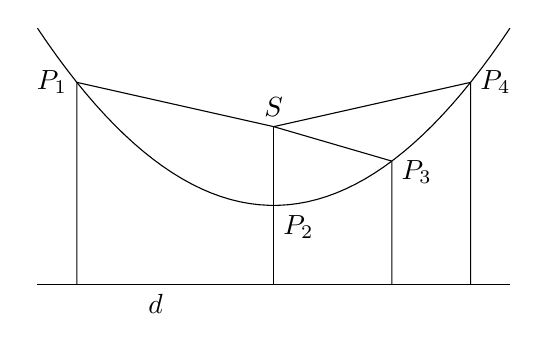
\begin{tikzpicture}[scale=.5]

% Construct focus and directrix and plot the parabola
\coordinate (F) at (0,2);
\node[above] at (F) {$S$};
\draw (-6,-2) -- node[below,near start] {$d$} (6,-2);
\draw[domain=-6:6,samples=50] plot (\x,{\x*\x/8});

% Locate Ps and label
\coordinate (P1) at (-5,3.125);
\coordinate (P2) at (0,0);
\coordinate (P3) at (3,1.125);
\coordinate (P4) at (5,3.125);

\node[left] at (P1) {$P_1$};
\node[below right] at (P2) {$P_2$};
\node[right,yshift=-4pt] at (P3) {$P_3$};
\node[right] at (P4) {$P_4$};

% Draw lines from focus to Ps and then to the directrix
\draw (F) -- (P1) -- (-5,-2);
\draw (F) -- (P2) -- (0,-2);
\draw (F) -- (P3) -- (3,-2);
\draw (F) -- (P4) -- (5,-2);
\end{tikzpicture}
\end{center}
\caption{A parabola defined by the focus and the directrix}\label{f.parabola}
\end{figure}

\begin{definition}
Let $X$ be the intersection of the perpendicular to the directrix from $S$. $A$ on $SX$ is a \emph{vertex} of the ellipse if $SA/AX=e$ (in Figure~\ref{f.def-ellipse}, $e=1/2$).
\end{definition}

%%%%%%%%%%%%%%%%%%%%%%%%%%%%%%%%%%%%%%%%%%%%%%%%%%%%%%%%%%

\begin{figure}[b]
\begin{center}
\begin{tikzpicture}

% Construct the directrix and the focus
\coordinate (X) at (0,0);
\node[left] at (X) {$X$};
\draw[name path=directrix] ($(X)+(0,2)$) --
  node[left,near start] {$d$} ($(X)+(0,-2)$);
\coordinate (S) at (3,0);
\node[below] at (S) {$S$};

% Locate the vertices with eccentricity 1/2
\coordinate (A) at (2,0);
\node[below] at (A) {$A$};
\coordinate (AP) at (9,0);
\node[below] at (AP) {$A'$};

% draw the major axis
\draw  (AP) -- node[above] {$6$} (S) -- 
  node[above left] {$1$} (A) -- node[above] {$2$} (X);

%\vertexsm{X};
\vertexsm{S};
\vertexsm{A};
\vertexsm{AP};
\end{tikzpicture}
\end{center}
\caption{The elements of the definition of an ellipse}\label{f.def-ellipse}
\end{figure}

%%%%%%%%%%%%%%%%%%%%%%%%%%%%%%%%%%%%%%%%%%%%%%%%%%%%%%%%%%
\vspace*{-5ex}

\subsubsection*{Constructing the vertices}

Given $e=SA/AX$ we can locate $A$ as follows:
\begin{eqn}
SA+AX&=&SX\\[4pt]
SA&=&SX\cdot \frac{e}{1+e}\\[4pt]
AX&=&SX\cdot \frac{1}{1+e}\,.
\end{eqn}
Similarly, there is a second vertex $A'$ where
\begin{eqn}
A'X-SA'&=&SX\\[4pt]
SA'&=&SX\cdot \frac{1}{1-e}\\[4pt]
A'X&=&SX\cdot \frac{2-e}{1-e}\,.
\end{eqn}

%%%%%%%%%%%%%%%%%%%%%%%%%%%%%%%%%%%%%%%%%%%%%%%%%%%%%%%%%%

\subsubsection*{Constructing points on an ellipse}

Select an \emph{arbitrary} point $E$ on the directrix and construct lines from $E$ through $A$ and $S$. The line through $S$ will make an angle $\alpha$ with $SX$. Construct a line from $S$ at the \emph{same angle} $\alpha$ from $ES$ and let its intersection with $EA$ be $P$. Construct the perpendicular from $P$ to the directrix and let $K$ be its intersection with the directrix. Let $L$ be the intersection of $KP$ with $ES$ (Figure~\ref{f.construct}). 

%%%%%%%%%%%%%%%%%%%%%%%%%%%%%%%%%%%%%%%%%%%%%%%%%%%%%%%%%%

\begin{figure}[t]
\begin{center}
\begin{tikzpicture}[scale=1.2]

\clip (-1,-2) rectangle +(9,4.5);

% Construct the directrix, the focus and the major axis
\coordinate (X) at (0,0);
\node[left] at (X) {$X$};
\draw[name path=directrix] ($(X)+(0,2.2)$) --
  node[left,near start] {$d$} ($(X)+(0,-2.2)$);
\coordinate (S) at (3,0);
\node[below right] at (S) {$S$};
\draw (X) -| ($(X)!2.4!(S)$) node[right] {$N$};

% Locate a vertex
\coordinate (A) at (2,0);
\node[above left] at (A) {$A$};

% Find a convenient E and draw _paths_ to A and S
\path[name path=findE] (S) -- +(210:4);
\path [name intersections = {of = findE and directrix, by = {E} }];
\node[left] at (E) {$E$};
\path[name path=EA] (E) -- ($(E)!2.3!(A)$);
\path[name path=ES] (E) -- ($(E)!2.3!(S)$);

% Locate P by drawing a path with the same angle
\path[name path=SP] (S) -- +(60:3);
\path [name intersections = {of = EA and SP, by = {P} }];
\node[above] at (P) {$P$};
\draw (S) -- (P);

% Construct the perpendicular through P to the directrix
\path[name path=PK] (P) -- +(180:4.5);
\path [name intersections = {of = PK and directrix, by = {K} }];
\node[left] at (K) {$K$};
\draw[name path=PL] (K) -- ($(K)!2!(P)$);

% Locate L and label the segments
\path [name intersections = {of = PL and ES, by = {L} }];
\node[above] at (L) {$L$};
\path (S) -- node[left] {$b$} (P) -- node[above] {$b$} (L);

% Label the angles
\node[right,xshift=12pt,yshift=5pt] at (S) {$\alpha$};
\node[above right,xshift=6pt,yshift=6pt] at (S) {$\alpha$};
\node[below left,xshift=-12pt,yshift=2pt] at (L) {$\alpha$};

% Draw the colored triangles
\draw[red,very thick] (P) -- (L) -- (E) -- cycle;
\draw[blue,very thick] (E) -- (K) -- ($(P)+(-3pt,0)$) -- ($(E)+(0,3pt)$);

\end{tikzpicture}
\end{center}
\caption{Constructing points on the ellipse}\label{f.construct}
\end{figure}

%%%%%%%%%%%%%%%%%%%%%%%%%%%%%%%%%%%%%%%%%%%%%%%%%%%%%%%%%%

\begin{theorem}\label{thm.point-on-an-ellipse}
The point $P$ is on the ellipse.
\end{theorem}
\begin{proof}
$\angle PLS = \angle LSN=\alpha$ by alternate interior angles, so $\triangle LPS$ is isoceles and $PL=SP$. Since $PK\parallel SX$, $\triangle XEA\sim \triangle KEP$ and $\triangle AES\sim \triangle PEL$ are adjacent pairs of similar triangles, so
\[
\frac{PS}{PK}=\frac{PL}{PK}=\frac{SA}{AX}=e\,.
\]
Therefore, $P$ is on the ellipse.\hqed
\end{proof}

%%%%%%%%%%%%%%%%%%%%%%%%%%%%%%%%%%%%%%%%%%%%%%%%%%%%%%%%%%

\begin{figure}[b]
\begin{center}
\begin{tikzpicture}[scale=1.1]

\clip (-1,-2) rectangle +(9,4.5);

% Construct directrix, focus and major axis
\coordinate (X) at (0,0);
\node[left] at (X) {$X$};
\draw[name path=directrix] ($(X)+(0,2.2)$) -- ($(X)+(0,-2.2)$);
\coordinate (S) at (3,0);
\node[below right] at (S) {$S$};
\draw (X) -| ($(X)!2.3!(S)$) node[right] {$N$};

% Locate O
\draw[name path=SP] (S) -- +(60:2) coordinate (P);
\node[above left] at (P) {$P$};

% Find a convenient F (but called E)
\path[name path=findE] (S) -- +(210:4);
\path [name intersections = {of = findE and directrix, by = {E} }];
\node[left] at (E) {$F$};

% Construct perpendicular through P from the directrix
\path[name path=PK] (P) -- +(180:4.5);
\path [name intersections = {of = PK and directrix, by = {K} }];
\node[left] at (K) {$K$};
\path[name path=PL] (K) -- ($(K)!2!(P)$);
\draw[name path=ES] (E) -- ($(E)!2!(S)$);
\path [name intersections = {of = PL and ES, by = {PP} }];
\node[above] at (PP) {$P'$};

% Draw triangles
\draw[blue,thick] (K) -- (S);
\draw[red,thick] (PP) -- (S) -- (P) -- cycle;
\draw[thick,dashed,red] (K) -- (P);

% Label angles
\draw[thick] ($(S)+(60:10pt)$)
  arc[start angle=60,end angle=210,radius=10pt];
\node[above,xshift=-4pt,yshift=8pt] at (S) {$\beta$};
\node[left,xshift=-18pt,yshift=6pt] at (S) {$\beta$};

\end{tikzpicture}
\end{center}
\caption{Constructing another vertex on $KP$}\label{f.other-vertex}
\end{figure}

%%%%%%%%%%%%%%%%%%%%%%%%%%%%%%%%%%%%%%%%%%%%%%%%%%%%%%%%%%

We now construct another point on $KP$. Construct a line from $F$ on the directrix through $S$ such that $\angle FSK = \angle KSP=\beta$ and let $P'$ be the intersection of $FS$ with $KP$ (Figure~\ref{f.other-vertex}).
\begin{theorem}
$P'$ is on the ellipse.
\end{theorem}

\enlargethispage{\baselineskip}
\begin{proof}
Since $KS$ bisects $\angle PSF$, by the exterior angle bisector theorem 
\begin{eqn}
\frac{SP'}{SP}&=&\frac{P'K}{PK}\\[4pt]
\frac{SP'}{P'K}&=&\frac{SP}{PK}=e\,,
\end{eqn}
and therefore $P$ is on the ellipse.\hqed
\end{proof}

%%%%%%%%%%%%%%%%%%%%%%%%%%%%%%%%%%%%%%%%%%%%%%%%%%%%%%%%%%

\subsection{Constructing a focal chord}

\begin{definition}
Let $P,P'$ be points on an ellipse. $PP'$ is a \emph{focal chord} of the ellipse if $PP'$ is a chord through a focus (Figure~\ref{f.focal-chord}).
\end{definition}

%%%%%%%%%%%%%%%%%%%%%%%%%%%%%%%%%%%%%%%%%%%%%%%%%%%%%%%%%%

\begin{figure}
\begin{center}
\begin{tikzpicture}[scale=1.4]

\clip (-.5,-2) rectangle +(8,4.2);

% Construct directrix, focus and major axis
\coordinate (X) at (0,0);
\node[left] at (X) {$X$};
\coordinate (S) at (3,0);
\node[below right] at (S) {$S$};
\path[name path=directrix] ($(X)+(0,2.2)$) -- ($(X)+(0,-2.2)$);
\draw (X) -| ($(X)!2.3!(S)$) node[right] {$N$};

% Locate a vertex
\coordinate (A) at (2,0);
\node[above left] at (A) {$A$};

% Find a convenient E and construct lines through A and S
\path[name path=findE] (S) -- +(210:4);
\path [name intersections = {of = findE and directrix, by = {E} }];
\node[left] at (E) {$E$};
\path[name path=EA] (E) -- ($(E)!2.3!(A)$);
\path[name path=ES] (E) -- ($(E)!2.3!(S)$);

% Locate P
\path[name path=SP] (S) -- +(60:3.5) coordinate (Q);
\path [name intersections = {of = EA and SP, by = {P} }];
\node[above] at (P) {$P$};

% Construct a perpendicular through P to the directrix
\path[name path=PK] (P) -- +(180:4.5);
\path [name intersections = {of = PK and directrix, by = {K} }];
\node[left] at (K) {$K$};

% Locate L
\draw[name path=PL] (K) -- ($(K)!1.8!(P)$);
\path [name intersections = {of = PL and ES, by = {L} }];
\node[above] at (L) {$L$};

% Draw triangle PLE and directrix
\draw (P) -- (L) -- (E) -- cycle;
\draw (E) -- (K);

% Locate A', P' and construct lines
\coordinate (AP) at (6,0);
\node[above] at (AP) {$A'$};
\draw[name path=EAP,very thick] (E) -- (AP);
\path[name path=SPP] (P) -- ($(P)!2!(S)$);
\path [name intersections = {of = SPP and EAP, by = {PP} }];
\draw[very thick] (P) -- (PP);
\node[below] at (PP) {$P'$};

% Locate K', L' and construct lines
\path[name path=PKP] (PP) -- +(-2.6,0);
\path [name intersections = {of = PKP and directrix, by = {KP} }];
\node[left] at (KP) {$K'$};
\draw[very thick] (PP) -- (KP);
\path [name intersections = {of = PKP and ES, by = {LP} }];
%\node[above,xshift=4pt,yshift=2pt] at (LP) {$L'$};

\node[above,xshift=-14pt,yshift=10pt] at (LP) {$L'$};

\draw[->] ($(LP)+(-10pt,8pt)$) -- +(-40:10pt);

% Label angles
\node[above right,xshift=13pt,yshift=-1pt] at (LP) {$\alpha$};
\node[below left,xshift=-7pt,yshift=-7pt] at (S) {$\alpha$};
\node[right,xshift=14pt,yshift=5pt] at (S) {$\alpha$};
\node[above right,xshift=8pt,yshift=8pt] at (S) {$\alpha$};
\node[below left,xshift=-14pt,yshift=1pt] at (L) {$\alpha$};

% Draw red and blue triangles
\draw[thick,red] (X) -- (S) -- (E);
\draw[thick,red] (KP) -- (LP);
\draw[thick,red] ($(E)+(-3pt,0)$) -- ($(S)+(-3pt,0)$);
\draw[thick,blue] (S) -- (AP) -- (E) -- cycle;
\draw[thick,blue] (LP) -- (PP);

\end{tikzpicture}
\end{center}
\caption{Constructing a focal chord}\label{f.focal-chord}
\end{figure}

%%%%%%%%%%%%%%%%%%%%%%%%%%%%%%%%%%%%%%%%%%%%%%%%%%%%%%%%%%

Let us continue with the construction of Figure~\ref{f.construct} as shown in Figure~\ref{f.focal-chord}. Construct the second vertex $A'$. Construct $EA'$ and label its intersection with $SP$ by $P'$. Construct a perpendicular from $P'$ to the directrix and label its intersection with the directrix by $K'$. Label the intersection of $P'K'$ and $EL$ by $L'$.
\begin{theorem}
The point $P'$ is on the ellipse and since $PP'$ intersects $S$ it is a focal chord.
\end{theorem}
\begin{proof}
$\triangle SEA' \sim \triangle L'EP'$ and $\triangle XES\sim K'EL'$ are adjacent similar triangles, so
\[
\frac{P'L'}{P'K'}=\frac{SA'}{A'X}\;.
\]
By alternate interior angles and vertical angles we have $\angle SL'P'=\angle L'SP'$ so triangle $\triangle SL'P'$ is isosceles and $P'L'=SP'$. Therefore,
\[
\frac{SP'}{P'K'}=\frac{SA'}{A'X}=e\,,
\]
and $P'$ is a point on the ellipse.\hqed
\end{proof}

%%%%%%%%%%%%%%%%%%%%%%%%%%%%%%%%%%%%%%%%%%%%%

\begin{figure}[b]
\begin{center}
\begin{tikzpicture}[scale=.9]

\clip (-1,-3.2) rectangle +(10.1,6.5);

% Construct ellipse
\draw[dashed,name path=ellipse] (5,0) ellipse[x radius=4,y radius={sqrt(8)}];

% Compute locations of P, P' on the ellipse 
\def\x{.5}
\def\y{sqrt((16-\x*\x)/2)}
\coordinate (P) at ({5+\x},{\y});
\node[above] at (P) {$P$};
\def\xp{-3.5}
\def\yp{-sqrt((16-\xp*\xp)/2)}
\coordinate (PP) at ({5+\xp},{\yp});
\node[right] at (PP) {$P'$};

% Construct focus and directrix
\coordinate (X) at (0,0);
\node[left] at (X) {$X$};
\path[name path=directrix] ($(X)+(0,3.3)$) -- ($(X)+(0,-3.3)$);
\coordinate (S) at ({5-sqrt(8)},0);
\node[right] at (S) {$S$};

% Locate F as extension of PP' to the directrix
\path[name path=PPP] (P) -- ($(P)!1.5!(PP)$);
\path[name intersections = {of = PPP and directrix, by = {F} }];
\node[left] at (F) {$F$};
\draw (PP) -- (F);

% Construct perpendiculars through K, K' to the directrix
\draw (P) -- (0,{\y}) coordinate (K);
\node[left] at (K) {$K$};
\draw[rotate=-90] (K) rectangle +(6pt,6pt);
\draw (PP) -- (0,{\yp}) coordinate (KP);
\node[left] at (KP) {$K'$};
\draw[rotate=-90] (KP) rectangle +(6pt,6pt);

% Draw triangles
\draw (S) -- (X) -- (F) -- (K);
\draw[thick,blue] (F) -- (S);
\draw[thick,red] (P) -- (S) -- (PP) -- cycle;
\draw[thick,red,dashed] (P) -- ($(P)!2!(S)$);

% Label angles
\node[xshift=20pt,yshift=-26pt] at (S) {$\beta$};
\node[xshift=-40pt,yshift=-26pt] at (S) {$\beta$};
\draw[->] ($(S)+(16pt,-26pt)$) -- +(180:32pt);
\draw[->] ($(S)+(-36pt,-26pt)$) -- +(0:14pt);

\end{tikzpicture}
\end{center}
\caption{Bisecting the angle at the focus}\label{f.bisect-angle}
\end{figure}

%%%%%%%%%%%%%%%%%%%%%%%%%%%%%%%%%%%%%%%%%%%%%%%%%%%%%

\begin{figure}[b]
\begin{center}
\begin{tikzpicture}[scale=1.1]

\clip (-1,-2) rectangle +(10,5.7);

% Construct the directrix and the focus
\coordinate (X) at (0,0);
\node[left] at (X) {$X$};
\path[name path=directrix] ($(X)+(0,4)$) -- ($(X)+(0,-2.2)$);
\coordinate (S) at (3,0);
\node[below right] at (S) {$S$};

% Locate the vertices
\coordinate (A) at (2,0);
\node[above left] at (A) {$A$};
\coordinate (AP) at (8,0);
\node[right] at (AP) {$A'$};

% Find a convenient E and construct paths through A, A', S
\path[name path=findE] (S) -- +(210:4);
\path[name intersections = {of = findE and directrix, by = {E} }];
\node[left] at (E) {$E$};
\path[name path=EA] (E) -- ($(E)!2.3!(A)$);
\path[name path=EAP] (E) -- ($(E)!1.1!(AP)$);
\path[name path=ES] (E) -- ($(E)!2!(S)$);

% Locate P, P' and draw EP
\path[name path=SP] (S) -- +(60:2.7) -- +(240:2.2);
\path[name intersections = {of = EA and SP, by = {P} }];
\node[above right] at (P) {$P$};
\path[name intersections = {of = EAP and SP, by = {PP} }];
\node[below] at (PP) {$P'$};
\vertexsmcolor{PP}{red};
\draw (E) -- (P);

% Locate F and draw lines
\path[name path=APF] (AP) -- ($(AP)!2.1!(P)$);
\path[name intersections = {of = APF and directrix, by = {F} }];
\draw (AP) -- (F) -- (E);
\node[left] at (F) {$F$};

% Draw blue angle and red triangle
\draw[name path=SF,thick,blue] (E) -- (S) -- (F);
\draw[red,thick] (P) -- (S) -- (AP) -- cycle;
\draw[red,thick,dashed] (PP) -- (S) -- (X);

% Label angles
\node[above,xshift=0pt,yshift=3pt] at (S) {$\gamma$};
\node[above left,xshift=-6pt,yshift=-1pt] at (S) {$\gamma$};
\node[below left,xshift=-16pt,yshift=1pt] at (S) {$\delta$};
\node[below,xshift=-16pt,yshift=-10pt] at (S) {$\delta$};

\draw[thick,blue,rotate=124] (S) rectangle +(5pt,5pt);

\end{tikzpicture}
\end{center}
\caption{The right angle at the focus}\label{f.right-angle}
\end{figure}

%%%%%%%%%%%%%%%%%%%%%%%%%%%%%%%%%%%%%%%%%%%%%%%%%%%%%%%%%%

\subsection{A right angle at the focus of an ellipse}

\begin{theorem}\label{thm.bisect}
Let $P,P'$ be points on the ellipse and let $F$ be the intersection of $PP'$ with the directrix. Then $FS$ bisects the exterior angle of $\angle P'SP$(Figure~\ref{f.bisect-angle}).
\end{theorem}
\begin{proof}
Since $P,P'$ are on the ellipse 
\[
\frac{SP}{PK}=\frac{SP'}{P'K'}=e\,,
\]
and since $\triangle PFK\sim P'FK'$,
\[
\frac{SP}{SP'}=\frac{PK}{P'K'}=\frac{PF}{P'F}\,.
\]
By the exterior angle bisector theorem $FS$ bisects the exterior angle of $\angle P'SP$.\hqed
\end{proof}

\begin{theorem}\label{thm.right-angle}
Let $P$ be a point on the ellipse and construct lines $PA,PA'$. Label their intersections with the directrix by $E$ and $F$, respectively. Then $\angle FSE$ is a right angle (Figure~\ref{f.bisect-angle}).
\end{theorem}

\begin{proof}
$P,A,A'$ are all points on the ellipse so Theorem~\ref{thm.bisect} applies. $FS$ bisects $\angle PSA=2\gamma$ and $ES$ bisects $\angle P'SA=2\delta$, so $2\gamma + 2\delta= 180^\circ$ and $\angle FSE=\gamma + \delta= 90^\circ$.\hqed
\end{proof}

%%%%%%%%%%%%%%%%%%%%%%%%%%%%%%%%%%%%%%%%%%%%%%%%%%%%%%%%%%%%%%%%

\subsection{Ratios}

\begin{theorem}\label{thm.ratios-besant}
Let $P$ be a point on an ellipse not on the major axis and construct perpendiculars $PN,PM$ from $P$ to the major and minor axes, respectively (Figure~\ref{f.besant-ratios}). Then
\begin{eqnlabels}
\frac{PN^2}{A'N\cdot AN}&=&\frac{BC^2}{AC^2} = \frac{b^2}{a^2}\label{eqn.pnan}\\[6pt]
\frac{PM^2}{B'N\cdot BN}&=&\frac{AC^2}{BC^2} = \frac{a^2}{b^2}\label{eqn.pmbn}\,.
\end{eqnlabels}
\end{theorem}

%%%%%%%%%%%%%%%%%%%%%%%%%%%%%%%%%%%%%%%%%%%%%%%%%%%%%%%%%%%%%%%%

\begin{proof} (Equation \ref{eqn.pnan})
$\triangle AXE\sim \triangle ANP$ since they are right triangles and the vertical angles at $A$ are equal (red). Therefore,
\begin{equation}
\frac{PN}{AN}=\frac{EX}{AX}\,.\label{eqn.triangle1}
\end{equation}
$\triangle PA'N\sim \triangle FA'X$ (blue) so
\begin{equation}
\frac{PN}{A'N}=\frac{FX}{A'X}\,.\label{eqn.triangle2}
\end{equation}
Multiplying Equations~\ref{eqn.triangle1} and \ref{eqn.triangle2} gives
\[
\frac{PN^2}{AN\cdot A'N}=\frac{EX\cdot FX}{AX\cdot A'X}\,.
\]
By Theorem~\ref{thm.right-angle} $\triangle FSE$ is a right triangle so by Theorem~\ref{thm.alt-hypo} giving
\[
\frac{PN^2}{AN\cdot A'N}=\frac{SX^2}{AX\cdot A'X}\,.
\]
Since $P$ was arbitrary this holds for any point on the ellipse, in particular, for $B$ on the minor axis, where $PN=BC$ and $AN=AN'=AC$. Therefore,
\begin{eqn}
\frac{BC^2}{AC^2}&=&\frac{SX^2}{AX\cdot A'X}\\[6pt]
\frac{PN^2}{AN\cdot A'N}&=&\frac{SX^2}{AX\cdot A'X}=\frac{BC^2}{AC^2}=\frac{b^2}{a^2}\,.\fqed
\end{eqn}
\end{proof}

%%%%%%%%%%%%%%%%%%%%%%%%%%%%%%%%%%%%%%%%%%%%%%%%%%%%%%%%%%%%%%%%

\begin{proof} (Equation \ref{eqn.pmbn})
From Equation~\ref{eqn.pnan}, since $CM=PN, PM=CN$ and by Theorem~\ref{thm.dividing},
\begin{eqnlabels}
AN\cdot NA'&=&AC^2-CN^2\\[6pt]
\frac{CM^2}{AC^2-PM^2}&=&\frac{BC^2}{AC^2}\nonumber\\[6pt]
\frac{AC^2}{AC^2-PM^2}&=&\frac{BC^2}{CM^2}\label{eqn.acbc1}\\[6pt]
\frac{AC^2}{PM^2}&=&\frac{BC^2}{BC^2-CM^2}\label{eqn.acbc2}\\[6pt]
\frac{PM^2}{BM\cdot MB'}&=&\frac{AC^2}{BC^2}\nonumber\,.
\end{eqnlabels}
The equivalence of Equations~\ref{eqn.acbc1}, \ref{eqn.acbc2} can be seen by cross-multiplying the equations.\hqed
\end{proof}

%%%%%%%%%%%%%%%%%%%%%%%%%%%%%%%%%%%%%%%%%%%%%%%%%%%%%%%%%%%%%%%%

\begin{figure}
\begin{center}
\begin{tikzpicture}[scale=.9]

\clip (-7,-2.5) rectangle +(12,7);

% Draw an hemi-ellipse with center C
\coordinate (C) at (0,0);
\node[below right] at (C) {$C$};
\def\a{4.33}
\def\b{3}
\draw[name path=ellipse] (\a,0) 
  arc[start angle=0,end angle=180, x radius=\a,y radius=\b];

% Locate a focal point
\coordinate (S) at ({-sqrt(\a*\a-\b*\b)},0);

% Draw axes
\coordinate (L) at +(180:{\a} and {\b});
\coordinate (R) at +(0:{\a} and {\b});
\node[below] at (R) {$A'$};
\node[above left] at (L) {$A$};
\coordinate (Top) at +(90:{\a} and {\b});
\node[above] at (Top) {$B$};
\draw[name path=major] (L) -- (R);
\draw[name path=minor] (C) -- (Top);
\draw[thick,dashed] (C) -- +(0,{-\b/3}) node[below] {$B'$};

% Construct directrix and focus
\coordinate (X) at (-6,0);
\node[left] at (X) {$X$};
\node[below right] at (S) {$S$};
\path[name path=directrix] ($(X)+(0,4.5)$) -- ($(X)+(0,-2.5)$);

% Locate P and E and draw lines
\path[name path=fromL] (L) -- +(50:4) -- +(230:3);
\path [name intersections = {of = ellipse and fromL, by = {P} }];
\node[above] at (P) {$P$};
\path [name intersections = {of = directrix and fromL, by = {E} }];
\node[left] at (E) {$E$};
\draw (P) -- (E);

% Locate F and draw lines
\path[name path=fromR] (R) -- ($(R)!1.7!(P)$);
\path [name intersections = {of = directrix and fromR, by = {F} }];
\node[left] at (F) {$F$};
\draw (R) -- (F);
\draw (F) -- (S) -- (E) -- cycle;
\draw[rotate=125] (S) rectangle +(7pt,7pt);

% Construct perpendiculars from P
\path (P) -- ($(L)!(P)!(C)$) coordinate (N) node[below] {$N$};
\draw (P) -- ($(Top)!(P)!(C)$) coordinate (M) node[right] {$M$};
\draw[rotate=180] (M) rectangle +(7pt,7pt);
\draw[rotate=90] (N) rectangle +(7pt,7pt);

% Draw red and blue similar triangles
\draw[thick,red] (X) -- (E) -- (P) -- (N) -- cycle;
\draw[thick,blue] ($(R)+(-4pt,2pt)$) -- ($(X)+(0,2pt)$) --
  (F) -- ($(F)!.99!(R)$);
\draw[thick,blue] ($(P)+(2pt,0)$) -- ($(P)!.98!($(N)+(2pt,0)$)$);

\end{tikzpicture}
\end{center}
\caption{Ratio of an ordinate}\label{f.besant-ratios}
\end{figure}

%%%%%%%%%%%%%%%%%%%%%%%%%%%%%%%%%%%%%%%%%%%%%%%%%%%%%%%%%%%%%%%%

\subsection{A circle circumscribing an ellipse}

Consider a circle of radius $a$ with the same center as an ellipse (Figure~\ref{f.ellipse-circle-besant}). Choose a point $N$ on the major axis and construct a perpendicular through $N$. Let its intersections with the ellipse and the circle be $P$ and $Q$, respectively.
\begin{theorem}\label{thm.ellipse-b-over-a-besant}
The perpendicular to the major axis through a point $Q$ on the circle circumscribing an ellipse intersects the ellipse at $P$ such that
\[
\frac{PN}{QN}=\frac{BC}{AC}=\frac{b}{a}\,.
\]
\end{theorem}
\begin{proof} 
From Theorem~\ref{thm.ratios-besant},
\[
\frac{PN^2}{AN\cdot NA'} = \frac{BC^2}{AC^2}\,,
\]
and by Theorem~\ref{thm.alt-hypo}, $AN\cdot NA=QN^2$.\hqed
\end{proof}

\begin{figure}[b]
\begin{center}
\begin{tikzpicture}[scale=.75]
\def\a{4.33}
\def\b{3}

% Draw a hemi-ellipse and a circumscribing hemi-circle
\coordinate (O) at (0,0);
\node[below] at (O) {$C$};
\draw[name path=circle] (\a,0)
  arc[start angle=0,end angle=180,radius=\a];
\draw[name path=ellipse] (\a,0)
  arc[start angle=0,end angle=180, x radius=\a,y radius=\b];

% Draw axes through O
\coordinate (L) at (-\a,0);
\coordinate (R) at (\a,0);
\coordinate (T) at (0,\a);
\draw[name path=major] (L) node[below] {$A$} -- (O) -- 
  (R) node[below] {$A'$};
\draw[name path=minor] (O) -- (T);
\path [name intersections = {of = minor and ellipse, by = {B} }];
\node[above right] at (B) {$B$};

% Choose arbitrary point on major-axis, raise a perpendicular
%   and label its intersections with the ellipse and the circle
\coordinate (N) at (-2,0);
\path[name path=atN] (N) -- ($(N)+(0,\a)$);
\path [name intersections = {of = atN and circle, by = {Q} }];
\draw (N) -- (Q);

% Label X and the intersections
\node[below] at (N) {$N$};
\node[above] at (Q) {$Q$};
\path [name intersections = {of = atN and ellipse, by = {P} }];
\node[above right] at (P) {$P$};

\end{tikzpicture}
\caption{A circle circumscribing an ellipse}\label{f.ellipse-circle-besant}
\end{center}
\end{figure}

%%%%%%%%%%%%%%%%%%%%%%%%%%%%%%%%%%%%%%%%%%%%%%%%%%%%%%%%%%%%%%%%

\subsection{The latus rectum of an ellipse}

\begin{definition}\label{def.ellipse-lr-besant}
Let $L=L_1L_2$ be a perpendicular to the major axis of an ellipse through a \emph{focus} $S$, such that its intersections with the ellipse are $L_1,L_2$. $L$ is a \emph{latus rectum} of an ellipse (Figure~\ref{f.ellipse-latus-rectum-besant}).\footnote{Normally, points are denoted by upper-case letters and line segments or lengths by lower-case letters, but $L$ for the latus rectum is the standard notation.}
\end{definition}

%%%%%%%%%%%%%%%%%%%%%%%%%%%%%%%%%%%%%%%%%%%%%%%%%%%%%%%%%%%%%%%%

\begin{figure}[t]
\begin{center}
\begin{tikzpicture}[scale=.75]

% Size and center of the ellipse
\def\a{4.33}
\def\b{3}

% Draw an ellipse with center C
\coordinate (C) at (0,0);
\node[below] at (C) {$C$};
\draw[name path=ellipse] (0,0) ellipse[x radius=\a, y radius=\b];

% The Sun is at a focal point
\coordinate (S) at ({-sqrt(\a*\a-\b*\b)},0);
\node[below right] at (S) {$S$};

% Draw axes
\coordinate (L) at (-\a,0);
\coordinate (R) at (\a,0);
\coordinate (B) at (0,-\b);
\coordinate (T) at (0,\b);
\node[above] at (T) {$B$};
\node[left] at (L) {$A$};
\node[right] at (R) {$A'$};
\draw (S) -- node[left] {$a$} (T);
\path (C) -- node[above] {$a$} (R);
\draw[name path=major] (L) -- (R);
\draw[name path=minor] (T) -- node[right] {$b$} (C);

% Locate intersections of LR with the ellipse and draw it
\path[name path=atS] (S) -- ($(S)+(0,3)$) -- ($(S)+(0,-3)$);
\path [name intersections = {of = atS and ellipse, by = {L,LP} }];
\node[above,yshift=2pt] at (L) {$L_1$};
\node[below] at (LP) {$L_2$};
\draw[thick,red] (L) -- (LP);

\end{tikzpicture}
\caption{The latus rectum of an ellipse}\label{f.ellipse-latus-rectum-besant}
\end{center}
\end{figure}

%%%%%%%%%%%%%%%%%%%%%%%%%%%%%%%%%%%%%%%%%%%%%%%%%%%%%%%%%%%%%%%%

\begin{theorem}\label{thm.ellipse-lr-besant}
$L$, the length of the latus rectum of an ellipse, is 
$\displaystyle\frac{2b^2}{a}$.
\end{theorem}
\begin{proof}
By Theorem~\ref{thm.ratios-besant},
\[
\frac{SL_1^2}{AS\cdot SA'}=\frac{BC^2}{AC^2}\,.
\]
By Theorem 7.2, $SB=AC=a$, so by Pythagoras's theorem,
\[
BC^2=BS^2-SC^2=AC^2-SC^2=(AC-SC)(AC+SC)=AS\cdot SA'\,.
\]
Therefore,
\begin{eqn}
SL_1^2&=&\frac{BC^4}{AC^2}\\[4pt]
SL_1&=&\frac{BC^2}{AC}=\frac{b^2}{a}\,,
\end{eqn}
but $L_1$ is one-half the latus rectum.\hqed
\end{proof}

%%%%%%%%%%%%%%%%%%%%%%%%%%%%%%%%%%%%%%%%%%%%%%%%%%%%%%%%%%%%%%%%

\subsection{Areas of parallelograms}

\begin{theorem}\label{thm.perp-tangent}
Let $Y$ be the intersection of the perpendicular to the focus $S$ and the tangent $TT'$ at $P$, and let $L$ be the intersection of $S'P$ and $SY$ (Figure~\ref{f.perp-focus-tangent}). Then $Y$ is on the circumscribing circle and $CY\parallel S'L$.
\end{theorem}

\begin{proof}
$\triangle STY$ and $\triangle T'TC$ are right triangles that share the acute angle $\angle CTT'=\angle YTS$ so $\angle CT'T=\angle YST$. $\angle SPY=\angle S'PT'$ by Theorem~\ref{thm.tangent-angles} since they are the angles to the foci at the tangent and $\angle S'PT'=\angle YPL$ are vertical angles so $\angle SPY=\angle SPT$. Then $\triangle SPY\cong\triangle SPT$ since they are right triangles with an equal acute angle and a common side $PY$. Therefore, $PL=PS$ and $S'L=S'P+PL=AA'=2a$.

Since $\triangle SPY\cong\triangle$, $SY=YL$, and since $S,S'$ are foci, $S'C=SC$. It follows that $\triangle CSY\sim \triangle S'SL$ and $CY\parallel S'L$. By similarity,
\[
\frac{CY}{S'L}=\frac{CS}{S'S}=\frac{CS}{2CS}\,.
\]
Therefore, $2CY=S'L=2a$ so $CY=a$ and $Y$ is on the circumscribing circle of radius $a$.\hqed
\end{proof}

%%%%%%%%%%%%%%%%%%%%%%%%%%%%%%%%%%%%%%%%%%%%%%%%%%%%%%

\begin{figure}[t]
\begin{center}
\begin{tikzpicture}

% Size and center of the ellipse
\def\a{4.33}
\def\b{3}
\coordinate (C) at (0,0);
\node[below] at (C) {$C$};

% Draw the ellipse and the circle
\draw[name path=ellipse] (\a,0) 
  arc[start angle=0,end angle=180,x radius=\a,y radius=\b];
\draw[thick,dotted] (\a,0) 
  arc[start angle=0,end angle=180,radius=\a];

% Locate the focal points
\coordinate (F1) at ({-sqrt(\a*\a-\b*\b)},0);
\node[below] at (F1) {$S'$};
\coordinate (F2) at ({+sqrt(\a*\a-\b*\b)},0);
\node[below] at (F2) {$S$};

% Draw axes AA' and BB'
\coordinate (L) at +(180:{\a} and {\b});
\coordinate (R) at +(0:{\a} and {\b});
\coordinate (Top) at +(90:{\a} and {\b});
\node[below] at (L) {$A'$};
\node[below] at (R) {$A$};
\draw[name path=major] (L) -- (R);
\draw (Top) -- (C);

% Select an arbitrary point P on the ellipse
\path[name path=fromF1p] (F1) -- +(25:8);
\path [name intersections = {of = ellipse and fromF1p, by = {P} }];
\node[above,xshift=0pt,yshift=0pt] at (P) {$P$};

% Draw tangent at P and locate its intersections with the axes
\tkzDefLine[bisector out](F1,P,F2) \tkzGetPoint{Tan1}
\path[name path=t1] ($(Tan1)!-.5!(P)$) coordinate (Z) -- 
  ($(Tan1)!1.75!(P)$) coordinate (TP);
\path[name path=ct] (C) -- ($(C)!2!(R)$);
\path[name path=bt] (C) -- ($(C)!1.5!(Top)$);
\path [name intersections = {of = t1 and bt, by = {TP} }];
\path [name intersections = {of = t1 and ct, by = {T} }];
\node[below] at (T) {$T$};
\node[above] at (TP) {$T'$};
\draw (C) -- (T) -- (TP) -- cycle;

% Construct the perpendicular through S to the tangent at Y
\draw (F2) -- ($(T)!(F2)!(TP)$) coordinate (Y);
\node[above] at (Y) {$Y$};
\draw[thick,dashed] (C) -- (Y);

% Construct lines through P and Y that meet in L
\path[name path=spp] (F1) -- ($(F1)!1.5!(P)$);
\path[name path=sy] (F2) -- ($(F2)!2.3!(Y)$);
\path [name intersections = {of = spp and sy, by = {LL} }];
\node[above left] at (LL) {$L$};
\draw (F1) -- (P) -- node[above] {$d$} (LL) -- 
  (F2) -- node[near start,left] {$d$} (P);

% Lable angles
\node[left,xshift=-3pt] at (P) {\sm{\alpha}};
\node[right,xshift=3pt] at (P) {\sm{\alpha}};
\node[below right,xshift=2pt,yshift=-2pt] at (P) {\sm{\alpha}};
\node[below right,xshift=2pt,yshift=-2pt] at (TP) {\sm{\beta}};
\node[above right,xshift=2pt,yshift=-2pt] at (F2) {\sm{\beta}};

\draw[rotate=-115]  (Y) rectangle +(7pt,7pt);
\draw  (C) rectangle +(7pt,7pt);

\end{tikzpicture}
\caption{The perpendicular from a focus to a tangent}\label{f.perp-focus-tangent}
\end{center}
\end{figure}

%%%%%%%%%%%%%%%%%%%%%%%%%%%%%%%%%%%%%%%%%%%%%%%%%%%%%%%%%%%%%%

\begin{theorem}\label{thm.cnntacac}
In Figure~\ref{f.segments-major}, $CN\cdot NT = AC^2=AN\cdot NA'$.
\end{theorem}

\begin{figure}[b]
\begin{center}
\begin{tikzpicture}

% Size and center of the ellipse
\def\a{4.33}
\def\b{3}
\coordinate (C) at (0,0);
\node[below] at (C) {$C$};

% Draw the ellipse
\draw[name path=ellipse] (\a,0) 
  arc[start angle=0,end angle=180, x radius=\a,y radius=\b];

% Locate the focal points
\coordinate (F1) at ({-sqrt(\a*\a-\b*\b)},0);
\node[below] at (F1) {$S'$};
\coordinate (F2) at ({+sqrt(\a*\a-\b*\b)},0);
\node[below] at (F2) {$S$};

% Draw axes AA' and BB'
\coordinate (L) at +(180:{\a} and {\b});
\coordinate (R) at +(0:{\a} and {\b});
\coordinate (Top) at +(90:{\a} and {\b});
\node[below] at (L) {$A'$};
\node[below] at (R) {$A$};
\draw[name path=major] (L) -- (R);
\draw (Top) -- (C);

% Select an arbitrary point P on the ellipse
\path[name path=fromF1p] (F1) -- +(25:8);
\path [name intersections = {of = ellipse and fromF1p, by = {P} }];
\node[above,xshift=0pt,yshift=0pt] at (P) {$P$};
\draw (F1) -- (P) -- (F2);

% Draw tangent at P and find its intersections with the axes
\tkzDefLine[bisector out](F1,P,F2) \tkzGetPoint{Tan1}
\path[name path=t1] ($(Tan1)!-.5!(P)$) coordinate (Z) -- 
  ($(Tan1)!1.75!(P)$) coordinate (TP);
\path[name path=ct] (C) -- ($(C)!2!(R)$);
\path[name path=bt] (C) -- ($(C)!1.5!(Top)$);
\path [name intersections = {of = t1 and bt, by = {TP} }];
\path [name intersections = {of = t1 and ct, by = {T} }];
\node[below] at (T) {$T$};
\node[above] at (TP) {$T'$};
\draw (C) -- (T) -- (TP) -- cycle;

% Locate perpendicular through focus to the tangent at Y
\draw (F2) -- ($(T)!(F2)!(TP)$) coordinate (Y);
\node[above] at (Y) {$Y$};

% Locate perpendicular through P to the major axis
\draw (P) --  ($(L)!(P)!(R)$) coordinate (N);
\node[below] at (N) {$N$};
\draw (N) -- (Y) -- (C);

% Label the angles
\node[left,xshift=-3pt] at (Y) {\sm{\alpha}};
\node[left,xshift=-3pt] at (P) {\sm{\alpha}};
\node[below right,xshift=1pt,yshift=-2pt] at (P) {\sm{\alpha}};
\node[above right,xshift=4pt,yshift=1pt] at (N) {\sm{\alpha}};

% Draw the triangles
\draw[thick,red] ($(Y)+(-1pt,-2pt)$) -- 
  ($(C)+(8pt,2pt)$) -- ($(T)+(-4pt,2pt)$) -- (Y);
\draw[thick,blue] (C) -- (N) -- (Y) -- cycle;

\draw[rotate=-115]  (Y) rectangle +(7pt,7pt);
\draw[rotate=90]  (N) rectangle +(7pt,7pt);

\end{tikzpicture}
\caption{Ratios of segments of the major axis}\label{f.segments-major}
\end{center}
\end{figure}

%%%%%%%%%%%%%%%%%%%%%%%%%%%%%%%%%%%%%%%%%%%%%%%%%%

\begin{proof}
Continuing with the construction from Figure~\ref{f.perp-focus-tangent}, we focus on the segments $AN,NA'$ (Figure~\ref{f.segments-major}). We can deduce the angles that are shown.
\begin{itemize}
\item $CY\parallel S'P$ (Theorem~\ref{thm.perp-tangent}) so $\angle CYP = \angle S'PT'$ by corresponding angles.
\item $\angle S'PT' = \angle SPY$ by Theorem~\ref{thm.tangent-angles} since they are the angles to the foci at the tangent.
\item $\angle SYP$ and $\angle SNP$ are right angles and therefore $SYPN$ is quadrilateral that can be circumscribed by a circle whose diameter is $PS$.
Therefore, $\angle SPY = \angle SNY$ since they are subtended by the same chord $YS$.
\end{itemize}
It follows that $\triangle CYT\sim \triangle CNY$ and
\begin{eqnlabels}
\frac{CN}{CY}&=&\frac{CY}{CT}\nonumber\\[6pt]
CN\cdot CT&=&CY^2=AC^2\,,\label{eqn.cnctacac}
\end{eqnlabels}
since the perpendicular to the tangent from a focus is on the circumscribing circle (Theorem~\ref{thm.perp-tangent}).

Since $NT=CT-CN$, we have $CN\cdot NT = CN\cdot CT - CN^2$ which equals $AC^2-CN^2$ by Equation~\ref{eqn.cnctacac}. This in turn equals $AN\cdot NA'$ by Theorem~\ref{thm.dividing}.\hqed
\end{proof}

%%%%%%%%%%%%%%%%%%%%%%%%%%%%%%%%%%%%%%%%%%%%%%%%%%%%%%%%%%%%%%

\begin{figure}[t]
\begin{center}
\begin{tikzpicture}[scale=.9]

% Size and center of the ellipse
\def\a{4.33}
\def\b{3}
\coordinate (C) at (0,0);
\node[below left,xshift=2pt] at (C) {$C$};

% Draw the ellipse
\draw[name path=ellipse] (C) ellipse[x radius=\a,y radius= \b];

% Locate the focal points
\coordinate (F1) at ({-sqrt(\a*\a-\b*\b)},0);
\coordinate (F2) at ({+sqrt(\a*\a-\b*\b)},0);

% Draw axes
\coordinate (L) at +(180:{\a} and {\b});
\coordinate (R) at +(0:{\a} and {\b});
\coordinate (Top) at +(90:{\a} and {\b});
\coordinate (Bot) at +(-90:{\a} and {\b});
\draw[name path=major] (L) -- 
  (R) node[below right] {$A$};
\draw[name path=minor] (Bot) --
  (Top) node[above left] {$B$};

% Select an arbitrary point P on the ellipse
\path[name path=fromF1p] (F1) -- +(20:8);
\path [name intersections = {of = ellipse and fromF1p, by = {P} }];
\path[name path=ph] (P) -- (F2);
\path[name path=pc] (P) -- (C);
\node[above,xshift=0pt,yshift=0pt] at (P) {$P$};

% Draw tangent at P and locate its intersections with the minor axis
\tkzDefLine[bisector out](F1,P,F2) \tkzGetPoint{Tan1}
\path[name path=t1] ($(Tan1)!.1!(P)$) coordinate (Z) -- 
  ($(Tan1)!1.75!(P)$) coordinate (TP);
\path[name path=bt] (C) -- ($(C)!1.5!(Top)$);
\path [name intersections = {of = t1 and bt, by = {T} }];
\node[left] at (T) {$T$};

% Conjugate diameters from D through C
\path[name path=cd] (C) -- +($(P)-(Z)$);
\path[name path=dk] (C) -- +($(Z)-(P)$);
\path [name intersections = {of = cd and ellipse, by = {D} }];
\path [name intersections = {of = dk and ellipse, by = {K} }];
\node[above left,xshift=3pt,yshift=-2pt] at (D) {$D$};
\node[below right,xshift=0pt,yshift=0pt] at (K) {$K$};
\draw (D) -- (K);

% Perpendicular through P on major axis and 
%   intersection with the conjugate diameter
\draw (P) -- ($(C)!(P)!(R)$) coordinate (N);
\node[below right] at (N) {$N$};
\path[name path=pk] (P) -- ($(P)!2!(N)$);
\path [name intersections = {of = pk and dk, by = {J} }];
\node[below left,yshift=4pt] at (J) {$J$};
\draw (N) -- (J);

% Locate normal to the tangent and its 
%   intersection with the conjugate diameter and the major axis
\draw[name path=pf] (P) -- ($(D)!(P)!(K)$) coordinate (F);
\node[below left] at (F) {$F$};
\path [name intersections = {of = pf and major, by = {G} }];
\node[above left] at (G) {$G$};

% Find intersection of tangent with the major axis
\path[name path=semimajor] (C) -- ($(C)!1.6!(R)$);
\path [name intersections = {of = t1 and semimajor, by = {TP} }];
\node[below] at (TP) {$T'$};
\draw (Top) -- (T) -- (TP) -- (R);

% Draw colored triangles and quadrilateral
\path[fill,black!10!white] (N) -- (G) -- (F) -- (J) -- cycle;
\draw[thick,red] (P) -- (N) -- (G) -- cycle;
\draw[thick,red] (C) -- (G) -- (F) -- cycle;
\draw[thick,blue] (C) -- (T) -- ($(TP)+(-3pt,2pt)$);
\draw[thick,blue] ($(TP)+(-3pt,2pt)$) -- ($(C)+(0,2pt)$);
\draw[thick,blue] ($(P)+(2pt,0)$) -- ($(N)+(2pt,0)$);

% Label angles
\node[above right,xshift=2pt,yshift=-1pt] at (G) {\sm{\alpha}};
\node[below left,xshift=-1pt,yshift=1pt] at (G) {\sm{\alpha}};
\node[below right,xshift=-4pt,yshift=0pt] at (G) {\sm{180^\circ\!-\!\alpha}};
\node[below right,xshift=10pt,yshift=3pt] at (C) {\sm{\beta}};
\node[above left,xshift=0pt,yshift=4pt] at (C) {\sm{\alpha}};
\node[below,xshift=-4pt,yshift=-6pt] at (P) {\sm{\beta}};
\node[below right,xshift=-2pt,yshift=-4pt] at (T) {\sm{\alpha}};
\node[above left,xshift=2pt,yshift=2pt] at (J) {\sm{\alpha}};

\draw[rotate=-32]  (F) rectangle +(7pt,7pt);
\draw[rotate=180]   (N) rectangle +(7pt,7pt);
\draw[rotate=-212] (P) rectangle +(7pt,7pt);
\draw[rotate=0]    (C) rectangle +(7pt,7pt);

\end{tikzpicture}
\caption{Parallelograms formed by conjugate diameters}\label{f.parallelogram-conjugate-diameters}
\end{center}
\end{figure}

%%%%%%%%%%%%%%%%%%%%%%%%%%%%%%%%%%%%%%%%%%%%%%%%%%%%%%%%%%%%%%

\begin{theorem}\label{thm.parallelogram1}
Construct the normal to the tangent at $P$ and let its intersection with the conjugate diameter $DK$ be $F$ and its intersection with the major axis be $G$. Construct a perpendicular from $P$ to the major axis and let its intersection be $N$ (Figure~\ref{f.parallelogram-conjugate-diameters}). Let the intersection of the tangent with the minor axis be $T$ and its intersection with the major axis be $T'$.
\[
PF\cdot PG = BC^2\,.
\]
\end{theorem}

%%%%%%%%%%%%%%%%%%%%%%%%%%%%%%%%%%%%%%%%%%%%%%%%%%%%%%%%%%%%%%

\begin{proof}
$\triangle NPG \sim \triangle FPJ$ (rotate $\triangle NPG$ to see this) so $\angle PGN=\angle PJF = \alpha$ and
\begin{eqn}
\frac{PF}{PN}&=&\frac{PJ}{PG}\nonumber\\[6pt]
PF\cdot PG &=& PJ\cdot PN\,.\label{eqn.pnpj}
\end{eqn}
By vertical angles $\angle PGN = \angle CGF = \alpha$ so 
$\triangle NPG\sim \triangle FCG$ and $\angle NPG = \angle FCG = \beta =90^\circ-\alpha$. By adding $\beta$ to the right angle $\angle BCN =\angle BNC$, we get that $\angle BCF = \angle BCJ$ and therefore $TPJC$ is a parallelogram, so $CT=PJ$ and $PF\cdot PG = CT\cdot PN$. We need to show that $CT\cdot PN=BC^2$.

$\triangle TT'C\sim \triangle PT'N$ so 
\begin{eqn}
\frac{CT}{CT'}&=&\frac{PN}{NT'}\\[6pt]
\frac{CT}{PN}&=&\frac{CT'}{NT'}\,.
\end{eqn}
Multiplying each side by fractions equal to $1$ gives
\[
\frac{CT\cdot PN}{PN^2}=\frac{CT'\cdot CN}{CN \cdot NT'}\,,
\]
and because ...
\[
\frac{CT\cdot PN}{PN^2}=\frac{AC^2}{AN\cdot NA'}\,.
\]
By Theorem~\ref{thm.ratios-besant} 
\begin{eqnlabels}
\frac{CT\cdot PN}{PN^2}&=&\frac{PN^2}{AN\cdot NA'}\cdot \frac{AC^2}{PN^2}=\frac{BC^2}{AC^2}\cdot \frac{AC^2}{PN^2}\nonumber\\[6pt]
CT\cdot PN&=&BC^2\,.\label{eqn.ctpn}\fqed
\end{eqnlabels}
\end{proof}

%%%%%%%%%%%%%%%%%%%%%%%%%%%%%%%%%%%%%%%%%%%%%%%%%%%%%%

\vspace*{-4ex}

\begin{theorem}\label{thm.cmpnacbc}
In Figure~\ref{f.parallelogram3},
\begin{eqn}
CN^2&=&AM\cdot MA',\quad CM^2=AN\cdot NA'\\[6pt]
\frac{DM}{CN}&=&\frac{BC}{AC}\\[6pt]
\frac{CM}{PN}&=&\frac{BC}{AC}
\end{eqn}
\end{theorem}

%%%%%%%%%%%%%%%%%%%%%%%%%%%%%%%%%%%%%%%%%%%%%%%%%%%%%%%%%%%%%%%%%%%%%%

\begin{figure}[t]
\begin{center}
\begin{tikzpicture}[scale=.8]

\clip (-8,-4) rectangle +(14,8);

% Size and center of the ellipse
\def\a{4.33}
\def\b{3}
\coordinate (C) at (0,0);
\node[below left,xshift=2pt,yshift=-4pt] at (C) {$C$};

% Draw the ellipse
\draw[name path=ellipse] (C) ellipse[x radius=\a,y radius= \b];

% Locate the focal points
\coordinate (F1) at ({-sqrt(\a*\a-\b*\b)},0);
\coordinate (F2) at ({+sqrt(\a*\a-\b*\b)},0);

% Draw axes
\coordinate (L) at +(180:{\a} and {\b});
\coordinate (R) at +(0:{\a} and {\b});
\coordinate (Top) at +(90:{\a} and {\b});
\coordinate (Bot) at +(-90:{\a} and {\b});
\draw[name path=major] (L) node[below left] {$A'$} --
  (R) node[below right] {$A$};
\draw[name path=minor] (Bot) node[below] {$B'$} --
  (Top) node[above] {$B$};

% Select an arbitrary point P on the ellipse
\path[name path=fromF1p] (F1) -- +(15:9);
\path [name intersections = {of = ellipse and fromF1p, by = {P} }];
\path[name path=ph] (P) -- (F2);
\draw[name path=pc] (P) -- (C);
\node[above right] at (P) {$P$};

% Draw tangent at P and locate intersection
%  with the extension of the major axis
\path[name path=tans] ($(L)+(-4,0)$) -- ($(R)+(2,0)$);
\tkzDefLine[bisector out](F1,P,F2) \tkzGetPoint{Tan1}
\path[name path=t1] (P) -- ($(Tan1)!.2!(P)$) coordinate (Z);
\path [name intersections = {of = t1 and tans, by = {T} }];
\node[below] at (T) {$T$};
\draw (P) -- (T);

% Diameter from P through C
\draw[name path=pc] (P) -- ($(P)!2!(C)$) coordinate (G);
\node[below left] at (G) {$P'$};

% Conjugate diameter from D through C
\path[name path=cd] (C) -- +($(P)-(Z)$);
\path[name path=dk] (C) -- +($(Z)-(P)$);
\path [name intersections = {of = cd and ellipse, by = {D} }];
\path [name intersections = {of = dk and ellipse, by = {K} }];
\node[above left] at (D) {$D$};
\node[below right] at (K) {$K$};
\draw (D) -- (K);

% Draw tangent at D and locate intersection with the major axis
\tkzDefLine[bisector out](F1,D,F2) \tkzGetPoint{Tan3}
\path[name path=t3] (D) --  ($(Tan3)!4.3!(D)$);
\path [name intersections = {of = tans and t3, by = {TP} }];
\draw (D) -- (TP) node[below] {$T'$};
\draw (T) -- (TP);

% Construct perpendiculars from P, D to the major axis
\draw (P) -- ($(L)!(P)!(R)$) coordinate (N) node[below] {$N$};
\draw (D) -- ($(L)!(D)!(R)$) coordinate (MM) node[below] {$M$};

\draw[rotate=90]   (N) rectangle +(8pt,8pt);
\draw[rotate=0]    (MM) rectangle +(8pt,8pt);

\end{tikzpicture}
\caption{Ratios of perpendiculars to the major axis}\label{f.parallelogram3}
\end{center}
\end{figure}

%%%%%%%%%%%%%%%%%%%%%%%%%%%%%%%%%%%%%%%%%%%%%%%%%%%%%%

\begin{proof}
By Theorem~\ref{thm.cnntacac},
\begin{eqn}
CN\cdot CT &=& AC^2=CM\cdot CT'\\[6pt]
\frac{CM}{CN} &=& \frac{CT}{CT'}\,.
\end{eqn}
Since $DK$ and $PP'$ are conjugate diameters, $DT'\parallel PP'$ and $\triangle T'DC \sim \triangle CPT$, so
\begin{eqn}
\frac{CM}{CN} &=& \frac{CT}{CT'} =  \frac{CN}{MT'}\\[6pt]
CN^2 &=& CM\cdot MT'\,,
\end{eqn}
Therefore,
\begin{equation}
CN^2=CM\cdot MT'=AC^2-CM^2 = AM\cdot MA'\label{eqn.cnannap}
\end{equation}
by Theorem~\ref{thm.cnntacac}. By Theorem~\ref{thm.ratios-besant},
\[
\frac{DM^2}{AM\cdot MA'}=\frac{BC^2}{AC^2}\,,
\]
and by Equation~\ref{eqn.cnannap},
\begin{eqn}
\frac{DM^2}{CN^2}&=&\frac{BC^2}{AC^2}\\[6pt]
\frac{DM}{CN}&=&\frac{BC}{AC}\,,
\end{eqn}
A symmetric argument shows that
\begin{eqn}
CM^2&=& AN\cdot NA'\\[6pt]
\frac{CM}{PN}&=&\frac{BC}{AC}\,\fqed.
\end{eqn}
\end{proof}

%%%%%%%%%%%%%%%%%%%%%%%%%%%%%%%%%%%%%%%%%%%%%%%%%%%%%%%%%%%%%%%%%%%%%%

\begin{theorem}\label{thm.area-parallelogram}
The area of the parallelogram formed by the tangents at the ends of the conjugate diameters $PG,DK$ is equal to the rectangle enclosing the ellipse at the ends of the axes (Figure~\ref{f.parallelogram2}).
\end{theorem}

\begin{proof}
By the definition of conjugate diameters, it is sufficient to show that the area of $PCDL$ is $AC\cdot BC$. The area of a parallelogram is width times height so it is $CD\cdot PF$. 

By vertical angles $\angle DCM = \angle GCF$ and $\angle CGF = \angle PGN$, so $\triangle DCM\sim \triangle PGN$ 
\[
\frac{PG}{CD}=\frac{PN}{CM}\,,
\]
and by Theorem~\ref{thm.cmpnacbc}
\begin{eqnlabels}
\frac{PG}{CD}&=&\frac{BC}{AC}\nonumber\\[6pt]
\frac{CD}{AC}&=&\frac{PG}{BC}\,.\label{eqn.cdac}
\end{eqnlabels}
By Theorem~\ref{thm.parallelogram1},
\begin{equation}
\frac{PG}{BC}=\frac{BC}{PF}\,.\label{eqn.pgbc}
\end{equation}
From Equations~\ref{eqn.cdac} and~\ref{eqn.pgbc} gives $CD\cdot PF = AC \cdot BC$.\hqed
\end{proof}

%%%%%%%%%%%%%%%%%%%%%%%%%%%%%%%%%%%%%%%%%%%%%%%%%%%%%%%%%%%%%%%%%%%%%%

\begin{figure}[t]
\begin{center}
\begin{tikzpicture}[scale=.8]

% Size and center of the ellipse
\def\a{4.33}
\def\b{3}
\coordinate (C) at (0,0);
\node[below left,xshift=2pt,yshift=-4pt] at (C) {$C$};

% Draw the ellipse
\draw[name path=ellipse] (C) ellipse[x radius=\a,y radius= \b];

% Locate the focal points
\coordinate (F1) at ({-sqrt(\a*\a-\b*\b)},0);
\coordinate (F2) at ({+sqrt(\a*\a-\b*\b)},0);

% Draw axes AA' and BB'
\coordinate (L) at +(180:{\a} and {\b});
\coordinate (R) at +(0:{\a} and {\b});
\coordinate (Top) at +(90:{\a} and {\b});
\coordinate (Bot) at +(-90:{\a} and {\b});
\draw[name path=major] (L) node[left] {$A'$} --
  (R) node[right] {$A$};
\draw[name path=minor] (Bot) node[below] {$B'$} --
  (Top) node[above] {$B$};

% Select an arbitrary point P on the ellipse
\path[name path=fromF1p] (F1) -- +(20:8);
\path [name intersections = {of = ellipse and fromF1p, by = {P} }];
\path[name path=ph] (P) -- (F2);
\path[name path=pc] (P) -- (C);
\node[above,xshift=0pt,yshift=0pt] at (P) {$P$};

% Draw tangent at P
\tkzDefLine[bisector out](F1,P,F2) \tkzGetPoint{Tan1}
\path[name path=t1] ($(Tan1)!.15!(P)$) -- ($(Tan1)!2!(P)$);

% Conjugate diameter from P through C
\draw[name path=pc] (P) -- ($(P)!2!(C)$) coordinate (G);
\node[below left] at (G) {$P'$};

% Find a point Z on tangent for drawing the tangent
\path[name path=f1q] (F1) -- +(60:6);
\path [name intersections = {of = f1q and t1, by = {Z} }];

% Conjugate diameters from D through C
\path[name path=cd] (C) -- +($(Z)-(P)$);
\path[name path=dk] (C) -- +($(P)-(Z)$);
\path [name intersections = {of = cd and ellipse, by = {D} }];
\path [name intersections = {of = dk and ellipse, by = {K} }];
\node[above left,xshift=1pt,yshift=-5pt] at (D) {$D$};
\node[below right,xshift=0pt,yshift=0pt] at (K) {$K$};
\draw (D) -- (K);

% Draw tangent at G (continuation of PC)
\tkzDefLine[bisector out](F2,G,F1) \tkzGetPoint{Tan2}
\path[name path=t2] ($(Tan2)!.1!(G)$) -- ($(Tan2)!1.9!(G)$);

% Draw tangent at D
\tkzDefLine[bisector out](F1,D,F2) \tkzGetPoint{Tan3}
\path[name path=t3] ($(Tan3)!-1.7!(D)$) -- ($(Tan3)!3.6!(D)$);

% Draw tangent at K (continuation of DC)
\tkzDefLine[bisector out](F1,K,F2) \tkzGetPoint{Tan4}
\path[name path=t4] ($(Tan4)!.2!(K)$)  -- ($(Tan4)!1.8!(K)$);

% Draw large dashed rectangle
\draw[thick,dashed] (\a,\b) -- (-\a,\b) -- 
  (-\a,-\b) -- (\a,-\b) -- cycle;

% Get the intersections of the tangents
\path [name intersections = {of = t1 and t3, by = {J} }];
\path [name intersections = {of = t2 and t3, by = {KK} }];
\path [name intersections = {of = t1 and t4, by = {M} }];
\path [name intersections = {of = t2 and t4, by = {LL} }];

% Draw the parallelogram
\draw (J) node[above] {$L$} -- (KK) -- (LL) -- (M) -- cycle;

% Locate perpendiculars of P, D with major axes
\draw (P) -- ($(L)!(P)!(R)$) coordinate (N) node[below] {$N$};
\draw (D) -- ($(L)!(D)!(R)$) coordinate (M) node[below] {$M$};

% Locate normal from P to the conjugate diameter
%   and its intersection with the major axes
\draw[name path=pf] (P) -- ($(D)!(P)!(K)$) coordinate (F);
\node[below left] at (F) {$F$};
\path [name intersections = {of = pf and major, by = {GG} }];
\node[above left] at (GG) {$G$};

% Draw colored triangles
\draw[thick,red]  (C) -- (M) --  (D) -- cycle;
\draw[thick,blue] (GG) -- (N) --  (P) -- cycle;

\draw[rotate=-32]  (F) rectangle +(7pt,7pt);
\draw[rotate=90]   (N) rectangle +(7pt,7pt);
\draw[rotate=-212] (P) rectangle +(7pt,7pt);
\draw[rotate=0]    (M) rectangle +(7pt,7pt);

\end{tikzpicture}
\caption{Areas of parallelograms}\label{f.parallelogram2}
\end{center}
\end{figure}

